\documentclass[uplatex, twocolumn, 10pt]{jsarticle} % Underfull \vbox (badness 10000) 文書の見た目が悪いらしいが、解決方法がよく分からない

\usepackage[dvipdfmx]{graphicx} % 画像処理に関するやつ
\usepackage{latexsym} % 数学の記述や論文作成などで頻繁に使用されるらしいやつ
\usepackage{bmpsize} % フォントのサイズ
\usepackage{url} % urlを扱うときに必要
\usepackage{comment} % 複数行のコメントができるらしいけど、#でいい気がする
% 余白の調整
% \usepackage[top=25truemm,bottom=25truemm,left=20truemm,right=20truemm]{geometry}
\setlength{\textheight}{636pt}
\setlength{\textwidth}{453pt}

% 使い方の例:\Underline{これが下線で強調されるテキストです。}\endUnderline
\def\Underline{\setbox0\hbox\bgroup\let\\\endUnderline} 
\def\endUnderline{\vphantom{y}\egroup\smash{\underline{\box0}}\\}

% コードの表示やコンピュータのファイル名、変数名などを強調するのに便利らしい(ソースはchatgpt)
\newcommand{\ttt}[1]{\texttt{#1}}

%%%  文書の最初  %%%
\begin{document}


% =================  タイトル  ====================
% 別な書き方
% \title{\bf
% {\LARGE{Codeless Web Testing using Selenium and Machine Learning\\
% Seleniumと機械学習を用いたコードレスWebテスト} \\ 
% \Large{Duyen Phuc Nguyen, Stephane Maag\\
% ICSOFT 2020: 15th International Conference on Software Technologies, Jul 2020, Online, France.
% pp.51-60}
% }}
\title{Translating Natural Language Requirements to Formal Specifications: A Study on GPT and Symbolic NLP \\
    自然言語要件の形式仕様への変換: GPTとシンボリックNLPに関する研究}
\author{Iat Tou Leong,  Raul Barbosa \\\\
    2023 53rd Annual IEEE/IFIP International Conference on Dependable Systems\\ and Networks Workshops (DSN-W), pp.259-262, June. 2023\\\\ 訳: 高橋 朋弘}
\date{2024年7月12日(金)}
\maketitle

% =================  概要  ====================
\section*{概要} % \section*は章番号をつけない
ソフトウェアの検証は信頼性を確保し、システムやコンポーネントが指定された要件を満たしていることを確認するために不可欠である。
自然言語は要件を指定する最も一般的な方法だが、定理証明などの多くの検証手法は、形式仕様記述言語で表された要件に依存している。
要件を自動的に形式仕様記述言語に変換することは、開発者が必要な専門知識を欠いていることが多いため、適切で挑戦的な研究課題である。
本研究では、上記の課題に対処するため、自然言語処理(NLP: Natural Language Processing)の適用を検討する。
本論文では、自然言語の要件を形式化するための2つの異なるアプローチ、シンボリックなアプローチとGPTベースのアプローチを考察する。
これら2つの方法は、テキスト要件から正確なJava Modeling Language(JML)を生成する能力に関して評価され、その結果は自動的な要件の形式化に対する大きな可能性を示した。

% =================  1.はじめに  ====================
\section{はじめに} % 1章
ソフトウェアの普及により、特に医療、航空宇宙、鉄道、自動車などの重要な分野において信頼性に関する懸念が高まっている。
そこで、ソフトウェアの信頼性を確保するため、ソフトウェア開発では正当性検証と妥当性確認を行う。
しかし、正当性検証と妥当性確認では、ソフトウェアの正確性を評価するために形式的な要件を必要とする。
静的チェックには通常、形式的な仕様が必要であり、動的テストには厳密な言語で記述したアサーションが必要である。

要件を形式化するには、厳密な構文と意味を持つ形式的な仕様言語に関する専門知識が必要である。
しかし、すべてのソフトウェア開発者がこの専門知識を持っているわけではない。
その結果、要件は自然言語で記述される場合が多くなる。
そのため、これらの要件を仕様言語に変換することが正当性検証と妥当性確認(V\&V)の重要な側面となる。

ソフトウェアの正確性を検証する場合、自然言語の要件を形式的な要件にする必要がある。
しかし、単語の意味は使用法によって異なることがある。
たとえば、「prime」という単語は日常生活では「supremacy(最上位)」を意味し、数学では1以外の因数を持たない数、すなわち素数を意味する。
意味の解釈を誤ると、壊滅的な結果を招く可能性がある。
加えて、要件を人手で変換するには労力と専門知識が必要となる。

本論文では、自然言語の要件をJava Modeling Language(JML)\cite{1}の形式的な要件に自動的に変換するために、自然言語処理(NLP: Natural Language Processing)を適用するという課題に取り組む。
具体的には、次の2つの異なるNLPアプローチを検討する。\\
1)ChatGPTを介してGPT\cite{2}を使用し、JMLに変換する方法。\\
2)著者らが設計したシンボリックアプローチで、ccg2lambda\cite{3}を使用して自然言語の要件から生成された高階論理意味表現を、コンパイラがJMLの形式的要件に変換する方法。\\
これらの2つの変換は、OpenJML\cite{4}とz3\cite{5}を使用して評価され、生成されたJMLの構文と意味の正確性、および生成されたJMLを使用したプログラムの正確性の両方が確認される。
本論文の全体的な目標は、自然言語の要件を演繹的検証に必要な形式要件に変換することで、ソフトウェア開発における時間とコストを大幅に節約する手段として、既存のNLP技術を研究することである。

本論文は以下のように構成される。
第\ref{sec:background}章では、本研究に関連する概念を簡単に紹介する。
第\ref{sec:approaches}章では、2つのアプローチについて説明する。
第\ref{sec:evaluation}章では、これらのアプローチのケーススタディを示す。
第\ref{sec:related_work}章では、関連する概念や文献を調査する。
第\ref{sec:conclusion}章では、結論を示す。

% =================  2. 背景  ====================
\section{背景}
\label{sec:background}
自然言語の要件を形式的な要件に自動的に変換することは、NLPを使用してテキスト要件を形式仕様記述言語に変換することを伴う。

\subsection{形式仕様記述言語}
形式仕様記述言語は、ソフトウェアを正確かつ明確であり、機械可読な方法で記述するために使用される言語である。
形式仕様化されたソフトウェアの正確性の検証では、定理証明を使用した演繹的検証などの手法が使用される。
JML仕様はJavaプログラムのコードコメント内に記述され、メソッドの動作仕様は//@で始まり、その後に事前条件のrequiresや事後条件のensuresなどのキーワードが続く。
また、数量詞(たとえば、forallやexists)やブール式を使用して、配列内の値がソートされているかを確認するなどの動作を指定することができる。
JMLではOpenJML\cite{4}やESC/Java\cite{6}など、演繹的検証を補助するツールを広く利用できる。

\subsection{自然言語処理}
自然言語処理(NLP)は、人間の言語を理解し解釈することができる計算モデルを開発することを目的とする研究分野である。
NLP は、言語の処理方法に基づいて、シンボリックアプローチと深層学習アプローチの2つのアプローチに大別できる。
シンボリックNLPは、単純な正規表現から複雑な文法までの明示的な表現と、言語の構文と意味を解釈するためのアルゴリズムを使用する\cite{3}。
一方、深層学習NLPは、深層ニューラルネットワークを使用して、大量のデータから言語のパターンや構造を学習する\cite{2}。

% =================  3. アプローチ  ====================
\section{アプローチ}
\label{sec:approaches}
JMLの形式的な要件を生成するため、シンボリックアプローチは著者らが設計したコンパイラに基づいており、深層学習アプローチはGPTに基づいている。

\subsection{シンボリックアプローチ}
コードコメントの入力テキスト要件に基づいて生成された意味表現を受け取り、図\ref{fig:Symb_app}に示すアプローチに従うコンパイラを構築した。
テキストに対し、NLPツールによって誤分類される可能性のある単語を置換するため、拡張可能なルールで前処理を行う。
たとえば、Javaのリテラルを表すキーワード(例: true, false, null)は、`a [keyword] value'(例: a true value)と置換する。
品詞タグ付けツールは通常、このような単語に対し形容詞としてタグ付けする。
しかし、これらの単語は一般的にブール値や、オブジェクト参照の比較で使用するため、名詞としてタグ付けする必要がある。

\begin{figure}[t]
    \begin{center}
        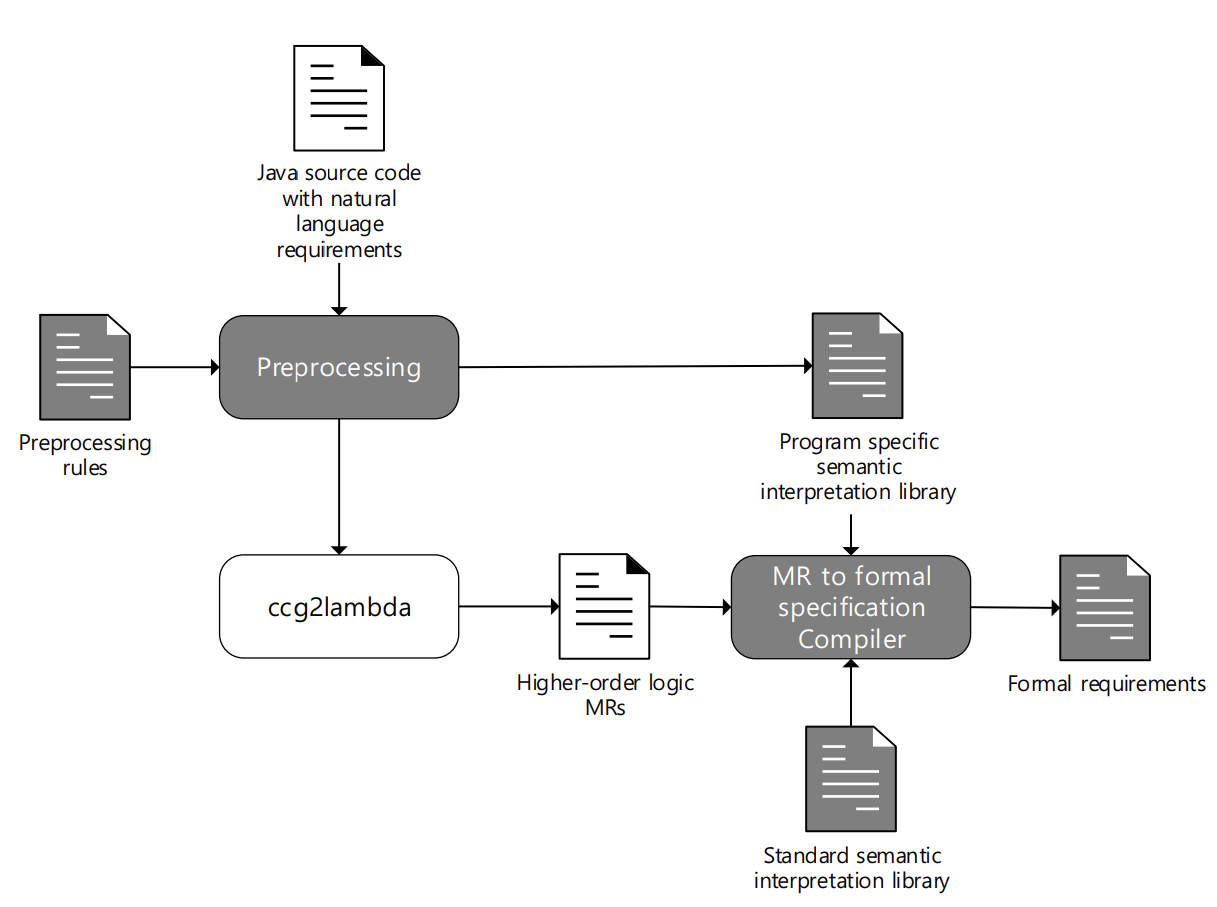
\includegraphics[width=\linewidth]{../image/TNLR/Fig1_Symb_app.png}
        \caption{テキスト要件の自動形式化に対する記号的アプローチ。
            高階論理意味表現は CCG 導出を通じて構築され、コンパイラはそれを JML に変換する。}
        \label{fig:Symb_app}
    \end{center}
\end{figure}

前処理された各文は、ccg2lambda\cite{3}を使用した変換プロセスを経る。
このプロセスには、トークン化、組み合わせカテゴリカル文法(CCG)木の導出、および意味構成が含まれる。
文は、区切り文字として空白を使用してトークン化される。
その後C\&Cパーサーによってタグ付けおよび解析がされ、CCG木が生成される。
葉とノードがNLTK\cite{7}ラムダ計算形式で記述されたテンプレートのルールと一致すると、ノード内の単語に意味を与え、高階論理意味表現を生成する。
そして、意味表現の向上のために、すべての 意味表現述語にそれぞれの構文カテゴリを注釈付けする。

Meaning Representation Compiler(MEARC)と名付けたコンパイラを設計および実装した。(https://github.com/itlchriss/MEARC)
このコンパイラは、意味表現を対応するJMLに変換するためのものである。
変換の中心的な概念は、構文カテゴリと引数を使用して、述語を意味解釈と一致させることである。
各意味解釈は、JML式を形成するために引数を受け入れるJML構造体である。
変換は、LR(1)文法で意味表現を解析することにより、抽象構文木を構築することから始まる。
抽象構文木の内部ノードは、接続詞(例: and(\&), or(\textbar))または述語である。
葉ノードは、述語の引数を表す変数である。

すべての述語ノードに分析を適用し、拡張可能な意味解釈ライブラリ内の意味解釈と一致させる。
述語ノードに一致する意味解釈がなく、またそれが別の述語の引数である場合は、意味解釈を提供する必要があることを示すエラーが発生する。
意味解釈を述語に対応付けした後、葉ノードを意味解釈の引数に代入することで、部分木から JML 構造体を合成する。
合成された JML 構造体は内部ノードに格納され、葉ノードは削除される。
最後に、木を後順で走査することにより、目的のJML を生成する。

\subsection{GPTアプローチ}
GPTモデル\cite{2}の学習は2段階に分けることができる。
第1段階は、明示的なラベル付けのない大規模なテキストコーパスでの教師なし事前学習プロセスである。
第2段階は、ラベル付けされたデータセットで学習を行い、特定のNLPタスクに適応させる教師ありファインチューニングプロセスである。
GPTモデルを変換に利用するために、ChatGPTを使用してクエリをモデルに入力する。
各クエリに対して、要件のJMLへの変換を明示的に要求し、モデルは追加の説明と共にJMLを提供する。

% =================  4. 評価と議論  ====================
\section{評価と議論}
\label{sec:evaluation}
それぞれのアプローチを評価するため、入力として 10 種類の要件を記述した。
GPT の場合、クエリとして``Please convert this sentence to JML: [requirement]"を使用した。
ここで、[requirement] はテキスト仕様である。
シンボリックアプローチとGPTの両方において、生成されたJMLに対しOpenJML\cite{4}を使用して構文と意味の正確性を確認する。
また、対応するJavaプログラムに関して静的に正確性を検証するため、OpenJMLとz3\cite{5}定理証明器を使用する。
以下の結果では、JML 仕様に対し、構文と意味のチェック、および z3 定理証明器による検証チェックを満たす場合にのみ正しいと見なす。

\begin{table*}[t]
    \caption{シンボリック NLP と GPT を使用して自然言語要件を JML に変換した結果}
    \label{tab:result_1}
    \centering
    \fontsize{6}{5}\selectfont
    \begin{tabular}{p{30mm}|p{45mm}|p{7mm}|p{45mm}|p{7mm}}
        \hline
        自然言語要件                                                                                       & シンボリックNLPで生成したJLM                                                                                                                                                                                                                                                                                                                                                                                                                                                                             & 正誤                                                             & GPTで生成したJLM                                                                                                                       & 正誤  \\
        \hline\hline
        1. The array should not be null.                                                                   & requires (array != null);                                                                                                                                                                                                                                                                                                                                                                                                                                                                                & 正                                                               & requires array != null;                                                                                                                & 正    \\ \hline
        2. If parameter x deeply equals parameter y, then result is true.                                  & ensures(((((x == null \&\& y == null) \&\& ((x == y) \textbar\textbar (x.equals(y)) \textbar\textbar Arrays.equals(x, y))) \textbar\textbar ((x != null \&\& y != null \&\& x.length == y.length) \&\& (\textbackslash forall int i; 0 \textless= i \textless x.length; ((x[i] == null \&\& y[i] == null) \textbar\textbar (x[i] != null \&\& y[i] != null \&\& (!x[i].getClass().isArray() \&\& !y[i].getClass().isArray() \&\& x[i].equals(y[i])))))))) ==\textgreater (\textbackslash result==true)); & 誤                                                               & requires x.deepEquals(y); \par ensures \textbackslash result == true;                                                                  & 誤    \\ \hline
        3. If and only if parameter x deeply equals parameter y, then result is true.                      & -                                                                                                                                                                                                                                                                                                                                                                                                                                                                                                        & 誤
                                                                                                           & requires x.deepEquals(y) \textless==\textgreater \textbackslash result == true;                                                                                                                                                                                                                                                                                                                                                                                                                          & 誤                                                                                                                                                                                                                \\ \hline
        4. If the input n is a prime number, the \par result is true.
                                                                                                           & ensures((n == 2 \textbar\textbar (n \textgreater 2 \&\& (\textbackslash forall int k; n \textgreater 2 \&\& 2 \textless= k \&\& k \textless= n/2; n \% k != 0))) ==\textgreater (\textbackslash result==true));
                                                                                                           & 正                                                                                                                                                                                                                                                                                                                                                                                                                                                                                                       & requires isPrime(n); \par ensures \textbackslash result == true; & 誤                                                                                                                                             \\ \hline
        5. If and only if the input n is prime, the result is true                                         & -                                                                                                                                                                                                                                                                                                                                                                                                                                                                                                        & 誤                                                               & requires isPrime(n) \textless==\textgreater \textbackslash result == true;                                                             & 誤    \\ \hline
        6. If the result is true, the input number is even                                                 & ensures((\textbackslash result==true) ==\textgreater (number \% 2 == 0));                                                                                                                                                                                                                                                                                                                                                                                                                                & 正                                                               & requires isEven(n) ==\textgreater \textbackslash result == true;                                                                       & 誤    \\ \hline
        7. If the result is false, the input number is not even                                            & ensures((\textbackslash result==false) ==\textgreater (!(number \% 2 == 0)));                                                                                                                                                                                                                                                                                                                                                                                                                            & 正                                                               & requires !isEven(n) ==\textgreater \textbackslash result == false;                                                                     & 誤    \\ \hline
        8. The input arr should be sorted in descending order                                              & ensures (\textbackslash forall int i; 0 \textless= i \&\& i \textless arr.length - 1; arr[i] \textgreater= arr[i + 1]);                                                                                                                                                                                                                                                                                                                                                                                  & 正                                                               & requires (\textbackslash forall int i, j; 0 \textless= i \&\& i \textless j \&\& j \textless arr.length; arr[i] \textgreater= arr[j]); & 正(?) \\ \hline
        9. The result is less than or equal to 2000 and the result is greater than or equal to 0.          & ensures((\textbackslash result \textgreater= 0) \&\& (\textbackslash result \textless= 2000));                                                                                                                                                                                                                                                                                                                                                                                                           & 正                                                               & ensures \textbackslash result \textgreater= 0 \&\& \textbackslash result \textless= 2000;                                              & 正    \\ \hline
        10. The input num1 is less than or equal to 1000 and the input num2 is less than or equal to 1000. & requires((num2 \textless= 1000) \&\& (num1 \textless= 1000));                                                                                                                                                                                                                                                                                                                                                                                                                                            & 正                                                               & requires num1 \textless= 1000 \&\& num2 \textless= 1000;                                                                               & 正    \\ \hline
    \end{tabular}
\end{table*}

自然言語要件に関する2つのアプローチの結果を表\ref{tab:result_1}に示す。
シンボリックアプローチは、10 回の翻訳のうち 7 回で正しい JML を生成した。
3行目と5行目では意味表現が誤って生成されたため、コンパイラからJMLが生成されなかった。
このような場合での意味表現導出を改善するためには、言語解釈のさらなる開発が必要である。
2行目については、生成された JML は 2つの配列の内容を比較しているが、Java の deep equals メソッドはネストされた配列の比較を実装するため、定理証明器によって拒否された。

GPTの結果に関しては、10件の変換のうち4件が完全に正しく、他にもいくつかはほぼ正解に近い結果だった。
2, 4, 5, 6, 7行目では、仕様で使用されているメソッドが存在しないか、その呼び出しが許可されていないため、変換が間違っている。
これは、GPT にコンテキスト情報が欠落しているために発生し、JML 仕様でセマンティック エラーが発生すると考えられる。
さらに、2行目の deepEquals メソッドの使用は構文的に誤っている (deepEquals メソッドは2つの引数を取る)。
3, 5, 6, 7行目では、事前条件で結果を参照しているため、構文エラーが発生している( `\textbackslash result'は`requires'句では許可されていない)。
全体として、以上の調査結果は、GPT ではJava API 仕様などの必要な知識を取得するために、特定の学習コーパスが必要であることを示している。

\begin{table*}[t]
    \caption{CHATGPT のクエリを変更した結果。元のクエリは``Please convert this sentence to JML: [requirement]"である。クエリに``without calling a separate function"を追加する変更を加えた。}
    \label{tab:result_2}
    \centering
    \fontsize{6}{5}\selectfont
    \begin{tabular}{p{25mm}|p{50mm}|p{55mm}|p{7mm}}
        \hline
        自然言語要件                                                   & 元のクエリから生成したJML                                             & 変更後のクエリから生成したJML                                                                                                                                                                                                                                    & 正誤 \\
        \hline\hline
        If parameter x deeply equals parameter y, then result is true. & requires x.deepEquals(y); \par ensures \textbackslash result == true; & ensures (\textbackslash result == true \&\& x.deepEquals(y)) \textbar\textbar (\textbackslash result == false \&\& !x.deepEquals(y));                                                                                                                            & 誤   \\ \hline
        If the input n is a prime number, the result is true.          & requires isPrime(n); \par ensures \textbackslash result == true;      & ensures (\textbackslash result == true \&\& (\textbackslash forall int i; 2 \textless= i \&\& i \textless n; n \% i != 0)) \textbar\textbar (\textbackslash result == false \&\& (\textbackslash exists int i; 2 \textless= i \&\& i \textless n; n \% i == 0)); & 正   \\ \hline
    \end{tabular}
\end{table*}

GPTの8行目の結果は議論の余地がある。
条件本体は正しく変換されている (つまり、降順でソートされていることを表す \textbackslash forall 句であること)。
しかし、変換されたJMLは事前条件であると見なしているが、おそらく事後条件であるべきである(メソッドが `result' を参照していないため)。
コンテキストを考慮しない場合、この要件はソートメソッドの事後条件またはバイナリ検索実装の事前条件である可能性がある。
このコンテキスト情報の重要性は、プログラムからコンテキスト情報を提供することで、深層学習アプローチを改善する研究の可能性を提示している
(たとえば、純粋なメソッドの void 戻り値の型は、引数を変更することを示唆している)。

仕様における誤ったメソッド呼び出しの問題をさらに調査するために、要件番号 2 と 4 の ChatGPT のクエリを変更し、``without calling a separate function(別の関数を呼び出さずに)"というフレーズを追加した。
表\ref{tab:result_2}に示す結果は、どちらの場合も生成された JML が`requires'を`ensures'に正しく置き換えていることを示している。
しかし、この置き換えはクエリを変更した際の目的ではなかった。
これにより、GPT によって提供される結果に非決定性があることが露呈した (これは既知の特性である)。
さらに、GPT は2つのクエリ間で一貫性のない方法でメソッド呼び出しを削除している。
`prime'の場合はメソッドの動作を正しく指定しているが、表\ref{tab:result_2}の最初の行にあるように、`deepEquals'の使用は残ったままになっている。

最後に、2つのアプローチを比較すると、GPT は自然言語文の意味をより正確に解釈できることが分かる。
しかし、Java API や言語の特性を完全には処理できない。
Java API のコーパスを具体的に使用してさらに学習することで、この点で GPT が改善される可能性がある。
また、結果はプログラムのコンテキスト情報やソフトウェアエンジニアリングの慣用句が変換プロセスにおいて重要な役割を果たしていることを示している。
したがって、シンボリックアプローチは言語解釈の点でより限定的であるが、言語が正しく解釈されれば、より正確な JML を提供する。

% =================  5. 関連研究  ====================
\section{関連研究}
\label{sec:related_work}
本論文では、自然言語の要件を自動的に形式化することに焦点を当てている。
既存のいくつかの手法では、構造化モデル\cite{8},\cite{9}、内部の事前定義ルール\cite{10}、モデルとヒューリスティックに基づく手法\cite{11},\cite{12}、分析とヒューリスティックに基づく手法\cite{13},\cite{14}、ロジックとそのパーサーの再定義\cite{15}のいずれかを使用し、
制限された自然言語セットを用いることで要件の自動形式化を実現している。
一方、本論文で使われている2つのアプローチは、自然言語入力に意図的な制限を課していない。

本論文で提示しているシンボリックアプローチは、ARSENAL\cite{16}に関連している。
ARSENAL は線形時相論理を生成するように設計されているが、ここで提示しているシンボリックアプローチは高階論理を処理できる。
結果として、線形時相論理は数量化をサポートしていないため、2つのアプローチの入力の複雑さは大きく異なる。
さらに、シンボリックアプローチで生成されるJML仕様は、定理証明を使用して検証を行うことができる。

FRET\cite{17}は、構造化された自然言語要件を形式化するアプローチであり、産業応用で有望な結果を示している。
しかし、FRETが受け入れる要件は数量化をサポートしていない。
また、制限のない自然言語要件をFRETで使用される構造化された自然言語要件に変換するため、GPTの使用を検討することは重要である。

% =================  6. 結論  ====================
\section{結論}
\label{sec:conclusion}
自然言語を使用してソフトウェアを分析することは、V\&V 技術を適用する組織にとって、時間とコストに関連する重要な課題である。
この課題に対処するための可能な解決策は、自然言語要件を正式な要件に変換し、演繹的検証を使用して変換された要件を評価することである。
本論文では、自然言語の要件を自動的に形式化する2つの異なる方法の実現可能性を評価した。
最初の方法は、ccg2lambda\cite{3}を利用して自然言語から得られた意味表現を形式要件に変換するシンボリックアプローチを採用している。
2つ目の方法は、GPT\cite{2}にクエリを送信することである。
どちらの方法も、目標言語として JML 仕様を生成できる。

一連の要件に対して2つのアプローチを評価し、シンボリックアプローチと GPT の両方が有意義で有望な結果をもたらすと結論付ける。
言語理解の点では、GPTは常にテキスト要件の意味を解釈するため、シンボリックアプローチよりも優れている。
ただし、シンボリックアプローチは、テキスト入力を解釈して意味表現を構築できる場合、JML を生成する際により正確である。
したがって、両方のアプローチは、自然言語要件の形式化を自動化し、形式手法を適用する労力を軽減する上で重要な貢献をすることができる。

\section*{訳者の感想}
自然言語からVDM仕様書を自動で生成するという研究に関連して、
LLMを用いて自然言語から仕様を生成している研究を調べたくてこの論文を読んだ。
LLMに関しての内容としては、「GPTを使ってJMLを生成してみた」といった程度だったが、従来のNLP手法との比較もあり参考になった。
この論文ではGPTを用いた仕様の生成について、GPTの自然言語に対する理解力の高さが述べられていた。
これより、自然言語からVDMを生成するにあたり、自然言語の分析部でGPTを活用できる可能性を考えた。
また、GPTでの生成に関する問題点として、Java API や言語の特性を完全に理解できていないことが挙げられていた。
実際に、Javaのメソッドを間違えて使っていたり、そもそもそのメソッドが使えるか分からない状態で呼び出していたりしていた。
これは、Javaに依存している問題であり、VDMではこのような問題は発生しない可能性があると考えた。
そのため、GPTはVDMであれば、高い精度で生成を行うことができる可能性があり、実際に試してみるべきであろうと考えた。
加えて、プロンプトについての考察も必要だと考えた。
この論文では、実際にプロンプトに一文追加しただけで、GPTの返答がかなり変わっていた。
これより、プロンプトに関する調査を行うことでも、精度の向上が見込めるだろうと考えた。
GPTで提供される結果の不安定性についても述べられていた。
この特性は大きな問題になりうるため、GPTを使用するのであれば、この特性への対応を考える必要があるだろうと考えた。

\begin{thebibliography}{99}
    \bibitem{1} G. T. Leavens, A. L. Baker, and C. Ruby, “Preliminary design of jml: A behavioral interface specification language for java,” SIGSOFT Softw. Eng. Notes, vol. 31, no. 3, p. 1-38, May 2006.
    \bibitem{2} A. Radford and K. Narasimhan, “Improving language understanding by generative pre-training,” 2018.
    \bibitem{3} P. Mart\'{i}nez-G\'{o}mez, K. Mineshima, Y. Miyao, and D. Bekki, “ccg2lambda: A compositional semantics system,” in Proceedings of ACL 2016 System Demonstrations. Berlin, Germany: Association for Computational Linguistics, August 2016, pp. 85-90.
    \bibitem{4} D. R. Cok, “OpenJML: JML for Java 7 by extending OpenJDK,” in NASA Formal Methods. Berlin, Heidelberg: Springer Berlin Heidelberg, 2011, pp. 472-479.
    \bibitem{5} L. de Moura and N. Bjørner, “Z3: An efficient smt solver,” in Tools and Algorithms for the Construction and Analysis of Systems, C. R. Ramakrishnan and J. Rehof, Eds. Berlin, Heidelberg: Springer Berlin Heidelberg, 2008, pp. 337-340.
    \bibitem{6} D. R. Cok and J. R. Kiniry, “Esc/java2: Uniting esc/java and jml,” in International Workshop on Construction and Analysis of Safe, Secure, and Interoperable Smart Devices. Springer, 2004, pp. 108-128.
    \bibitem{7} S. Bird, E. Klein, and E. Loper, Natural Language Processing with Python, 1st ed. O'Reilly Media, Inc., 2009.
    \bibitem{8} I. S. Bajwa, B. Bordbar, and M. G. Lee, “Ocl constraints generation from natural language specification,” in 2010 14th IEEE International Enterprise Distributed Object Computing Conf., 2010, pp. 204-213.
    \bibitem{9} C. Wang, F. Pastore, and L. Briand, “Automated generation of constraints from use case specifications to support system testing,” in 2018 IEEE 11th International Conference on Software Testing, Verification and Validation (ICST), 2018, pp. 23-33.
    \bibitem{10} A. Blasi, A. Goffi, K. Kuznetsov, A. Gorla, M. D. Ernst, M. Pezz\`{e}, and S. D. Castellanos, “Translating code comments to procedure specifications,” in Proceedings of the 27th ACM SIGSOFT International Symposium on Software Testing and Analysis, ser. ISSTA 2018. New York, NY, USA: Association for Computing Machinery, 2018, p. 242-253.
    \bibitem{11} Y. Zhou, R. Gu, T. Chen, Z. Huang, S. Panichella, and H. Gall, “Analyzing apis documentation and code to detect directive defects,” in 2017 IEEE/ACM 39th International Conference on Software Engineering (ICSE), 2017, pp. 27-37.
    \bibitem{12} J. Zhai, Y. Shi, M. Pan, G. Zhou, Y. Liu, C. Fang, S. Ma, L. Tan, and X. Zhang, C2S: Translating Natural Language Comments to Formal Program Specifications. New York, NY, USA: Association for Computing Machinery, 2020, p. 25-37.
    \bibitem{13} L. Tan, D. Yuan, G. Krishna, and Y. Zhou, “/*icomment: Bugs or bad comments?*/,” in Proceedings of Twenty-First ACM SIGOPS Symposium on Operating Systems Principles, ser. SOSP '07. New York, NY, USA: Association for Computing Machinery, 2007, p. 145-158.
    \bibitem{14} L. Tan, Y. Zhou, and Y. Padioleau, “Acomment: Mining annotations from comments and code to detect interrupt related concurrency bugs,” in Proceedings of the 33rd International Conference on Software Engineering, ser. ICSE '11. New York, NY, USA: Association for Computing Machinery, 2011, p. 11-20.
    \bibitem{15} C. Menghi, S. Nejati, K. Gaaloul, and L. C. Briand, “Generating automated and online test oracles for simulink models with continuous and uncertain behaviors,” in Proceedings of the 2019 27th ACM Joint Meeting on European Software Engineering Conference and Symposium on the Foundations of Software Engineering, ser. ESEC/FSE 2019. New York, NY, USA: Association for Computing Machinery, 2019, p. 27-38.
    \bibitem{16} S. Ghosh, D. Elenius, W. Li, P. Lincoln, N. Shankar, and W. Steiner, “Automatically extracting requirements specifications from natural language,” CoRR, vol. abs/1403.3142, 2014.
    \bibitem{17} M. Farrell, M. Luckcuck, O. Sheridan, and R. Monahan, “Fretting about requirements: Formalised requirements for an aircraft engine controller,” in Requirements Engineering: Foundation for Software Quality, V. Gervasi and A. Vogelsang, Eds. Cham: Springer International Publishing, 2022, pp. 96-111.
\end{thebibliography}

\end{document}